\section{Choix d'implémentation et variations effectuées}
Nous allons dans ce chapitre décrire les classes de notre programme afin d’une part clarifier le code, et d’autre part, facilité la modification et le contrôle.
\section{LunarPhysics}

\subsection{PhysicalObject}
Comme le dit son nom, cette classe s’occupe de créer un objet physique avec les paramètres suivants : la position initiale, la vitesse initiale, la largeur et la hauteur. Sur cet objet vont donc ensuite s’appliquer les forces physiques comme la force de gravité et la poussée des réacteurs. Cette classe implémente les interfaces Simulatable et Collisionable.

\subsection{PhysicsSimulator}
Cette classe représente pour nous la classe la plus difficile à implémenter et à comprendre. Elle contient :
\begin{enumerate}
\item La physique qui va agir sur les corps créer dans PhysicalObject
\item Les collisions entre les différents corps
\end{enumerate}

Concernant la physique nous avons choisis de représenter toutes les forces en Vector2, c’est-à-dire un vecteur où l’on donne les points en X et en Y comme paramètre. L’avantage de travailler avec les vecteurs est que toutes les informations concernant la force sont directement accessibles.

Les collisions ont été implémentées de la manière suivante : par exemple pour les collisions entre le paysage et le vaisseau spatial, nous avons créé une BoundingBox autour du vaisseau, c’est-à-dire un rectangle qui évite de devoir faire collisionner la forme compliquée du vaisseau. On a donc maintenant une collision entre un rectangle (vaisseau) et un polygone (paysage). Nous avons donc d’abord demandé si un des coins du rectangle se trouvait à l’intérieur du polygone (avec la méthode countains de PolygonWorking) et nous avons à ce moment là remarqué que si le vaisseau se posait sur un coin du polygone, les points du rectangle ne se trouvaient pas dans le polygone alors que le vaisseau aurait dû exploser. Nous avons donc ajouté une contrainte qui regarde si un point du polygone se trouve dans le rectangle. Les collisions se font correctement de cette manière.

\begin{figure}[h]
 \centering
 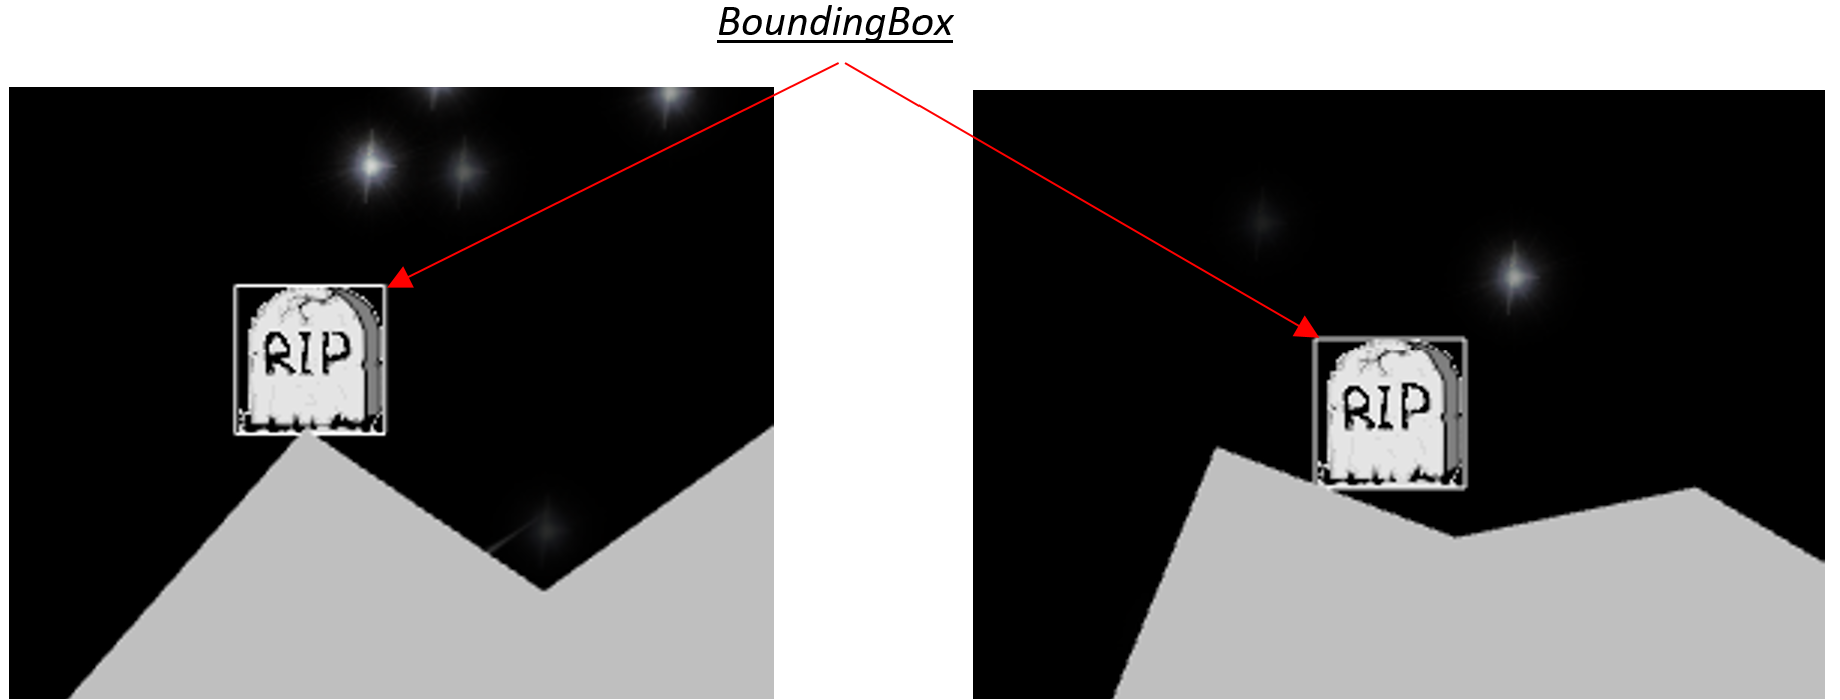
\includegraphics[width=0.75\linewidth]{Figures/BoundingBoxes.png}
 \caption{Collision entre un point du polygone et le rectangle et inversement}
 \label{figure:BoundingBoxes}
\end{figure}

Cette BoundingBox peut être activée et désactivée facilement dans les constantes.

\subsection{Simulatable}
Cette interface permet à chaque objet provenant d’une classe qui hérite de cette interface, d’avoir une méthode step qui va permettre de simuler chaque étape.

\subsection{Particles}
Voici le générateur de particule que nous avons créé à la suite d’un problème avec celui de GDX2D cité dans les problèmes dans ce rapport. Ces particules ont une durée de vie, une direction, une vitesse et une représentation graphique.

\subsection{Ground}
La classe Ground génère le sol de la lune. Il est représenté par un polygone. Lorsque l’on créer un objet Ground, le constructeur de cette classe va déterminer tous les points du polygone en utilisant des vecteurs qui partent tous du point (0,0). Une fois que tous les points sont créés, nous créons un objet. Cet objet va ensuite être affiché et utilisé pour les collisions.  PolygonWorking. Ensuite, nous avons la méthode getPolygon qui est appelée dans la classe main pour créer le polygone qui va ensuite s’afficher sur le jeu.
\begin{figure}[h]
 \centering
 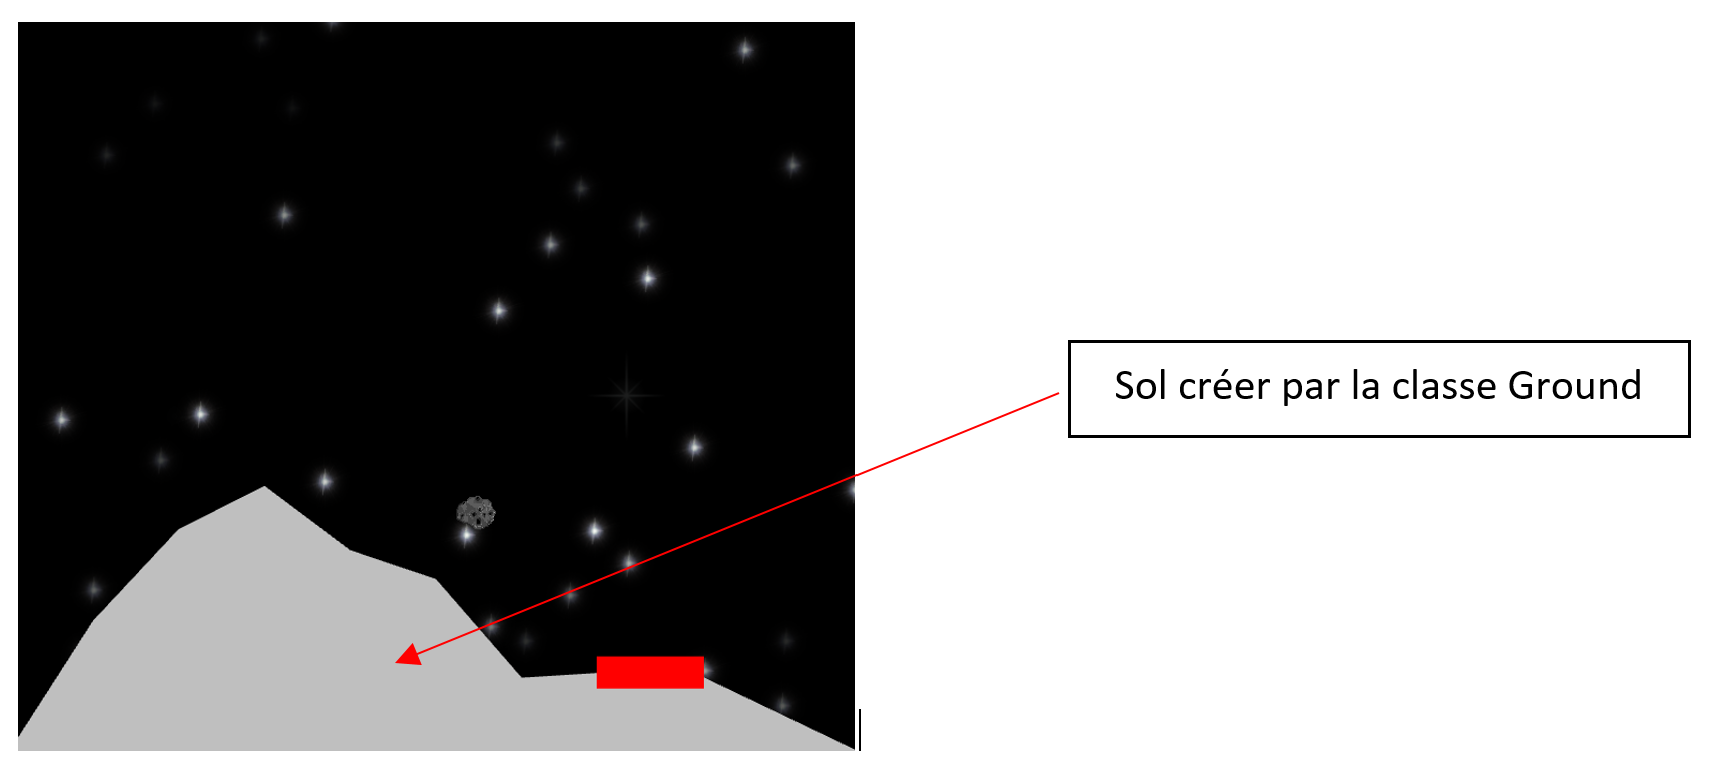
\includegraphics[width=0.75\linewidth]{Figures/Ground.png}
 \caption{Image d'illustration du polygone}
 \label{figure:Ground}
\end{figure}

\subsection{Constants}
Dans cette classe, nous avons mis toutes les constantes du jeu. Ceci nous permet et permet au prochain utilisateur de modifier simplement des variables dans le jeu sans pour autant devoir comprendre tout ce qui a été fait dans le code. C’est aussi un récapitulatif de nos paramètres utilisés et cela nous permet de garder un code propre.

\subsection{Collisionable}
Collisionnable est une interface qui s’occupe de voir quand est-ce qu’il y a une collision. C’est aussi dans cette interface qu’il y a les BoundingBox mentionnées ci-dessus. Cette interface nous a été fournie au début du projet.

\section{LunarMain}

\subsection{PolygonWorking}
Cette classe nous a aussi été fournie durant le projet. Elle hérite de la classe Polygon qui sert à créer un polygone. Pour créer une forme avec PolygonWorking, il faut appeler la fonction et donner en paramètre tous les points du polygone. Ces points sont donnés en vecteur.

\subsection{Gegner}

\subsection{LandZone}
Cette classe créer simplement un rectangle qui symbolise la zone d’atterrissage. Ce rectangle va être positionné à la position donnée par le vecteur en paramètre.

\subsection{SpaceShip}
C’est dans cette classe que nous créons le vaisseau. C’est aussi ici que nous faisons l’affichage de différents éléments dans la fenêtre comme la vitesse et le carburant restant. Nous initialisons aussi le fond noir de la fenêtre dans cette classe.

\subsection{LunarLander_Main}
